\chapter{Revisión de la literatura: estado del arte}
\label{chap:estado_arte}

Dentro de los algoritmos evolutivos, el uso de modelos subrogados surge como
respuesta a una limitación habitual en problemas de optimización costosa: la
evaluación repetida de la función objetivo. En este contexto, los algoritmos
evolutivos asistidos por subrogados (\textit{surrogate-assisted evolutionary
    algorithms}, SAEA) tratan de reducir el número de evaluaciones reales
necesarias mediante modelos aproximados que orientan la búsqueda hacia regiones
prometedoras.

La actividad reciente del área también se refleja en la evolución del número
de publicaciones indexadas en Scopus. La
Figura~\ref{fig:publicaciones_saea_scopus} muestra un crecimiento claro de los
trabajos relacionados con algoritmos evolutivos asistidos por subrogados
durante la última década, especialmente a partir de 2019.


\begin{figure}[H]
    \centering
    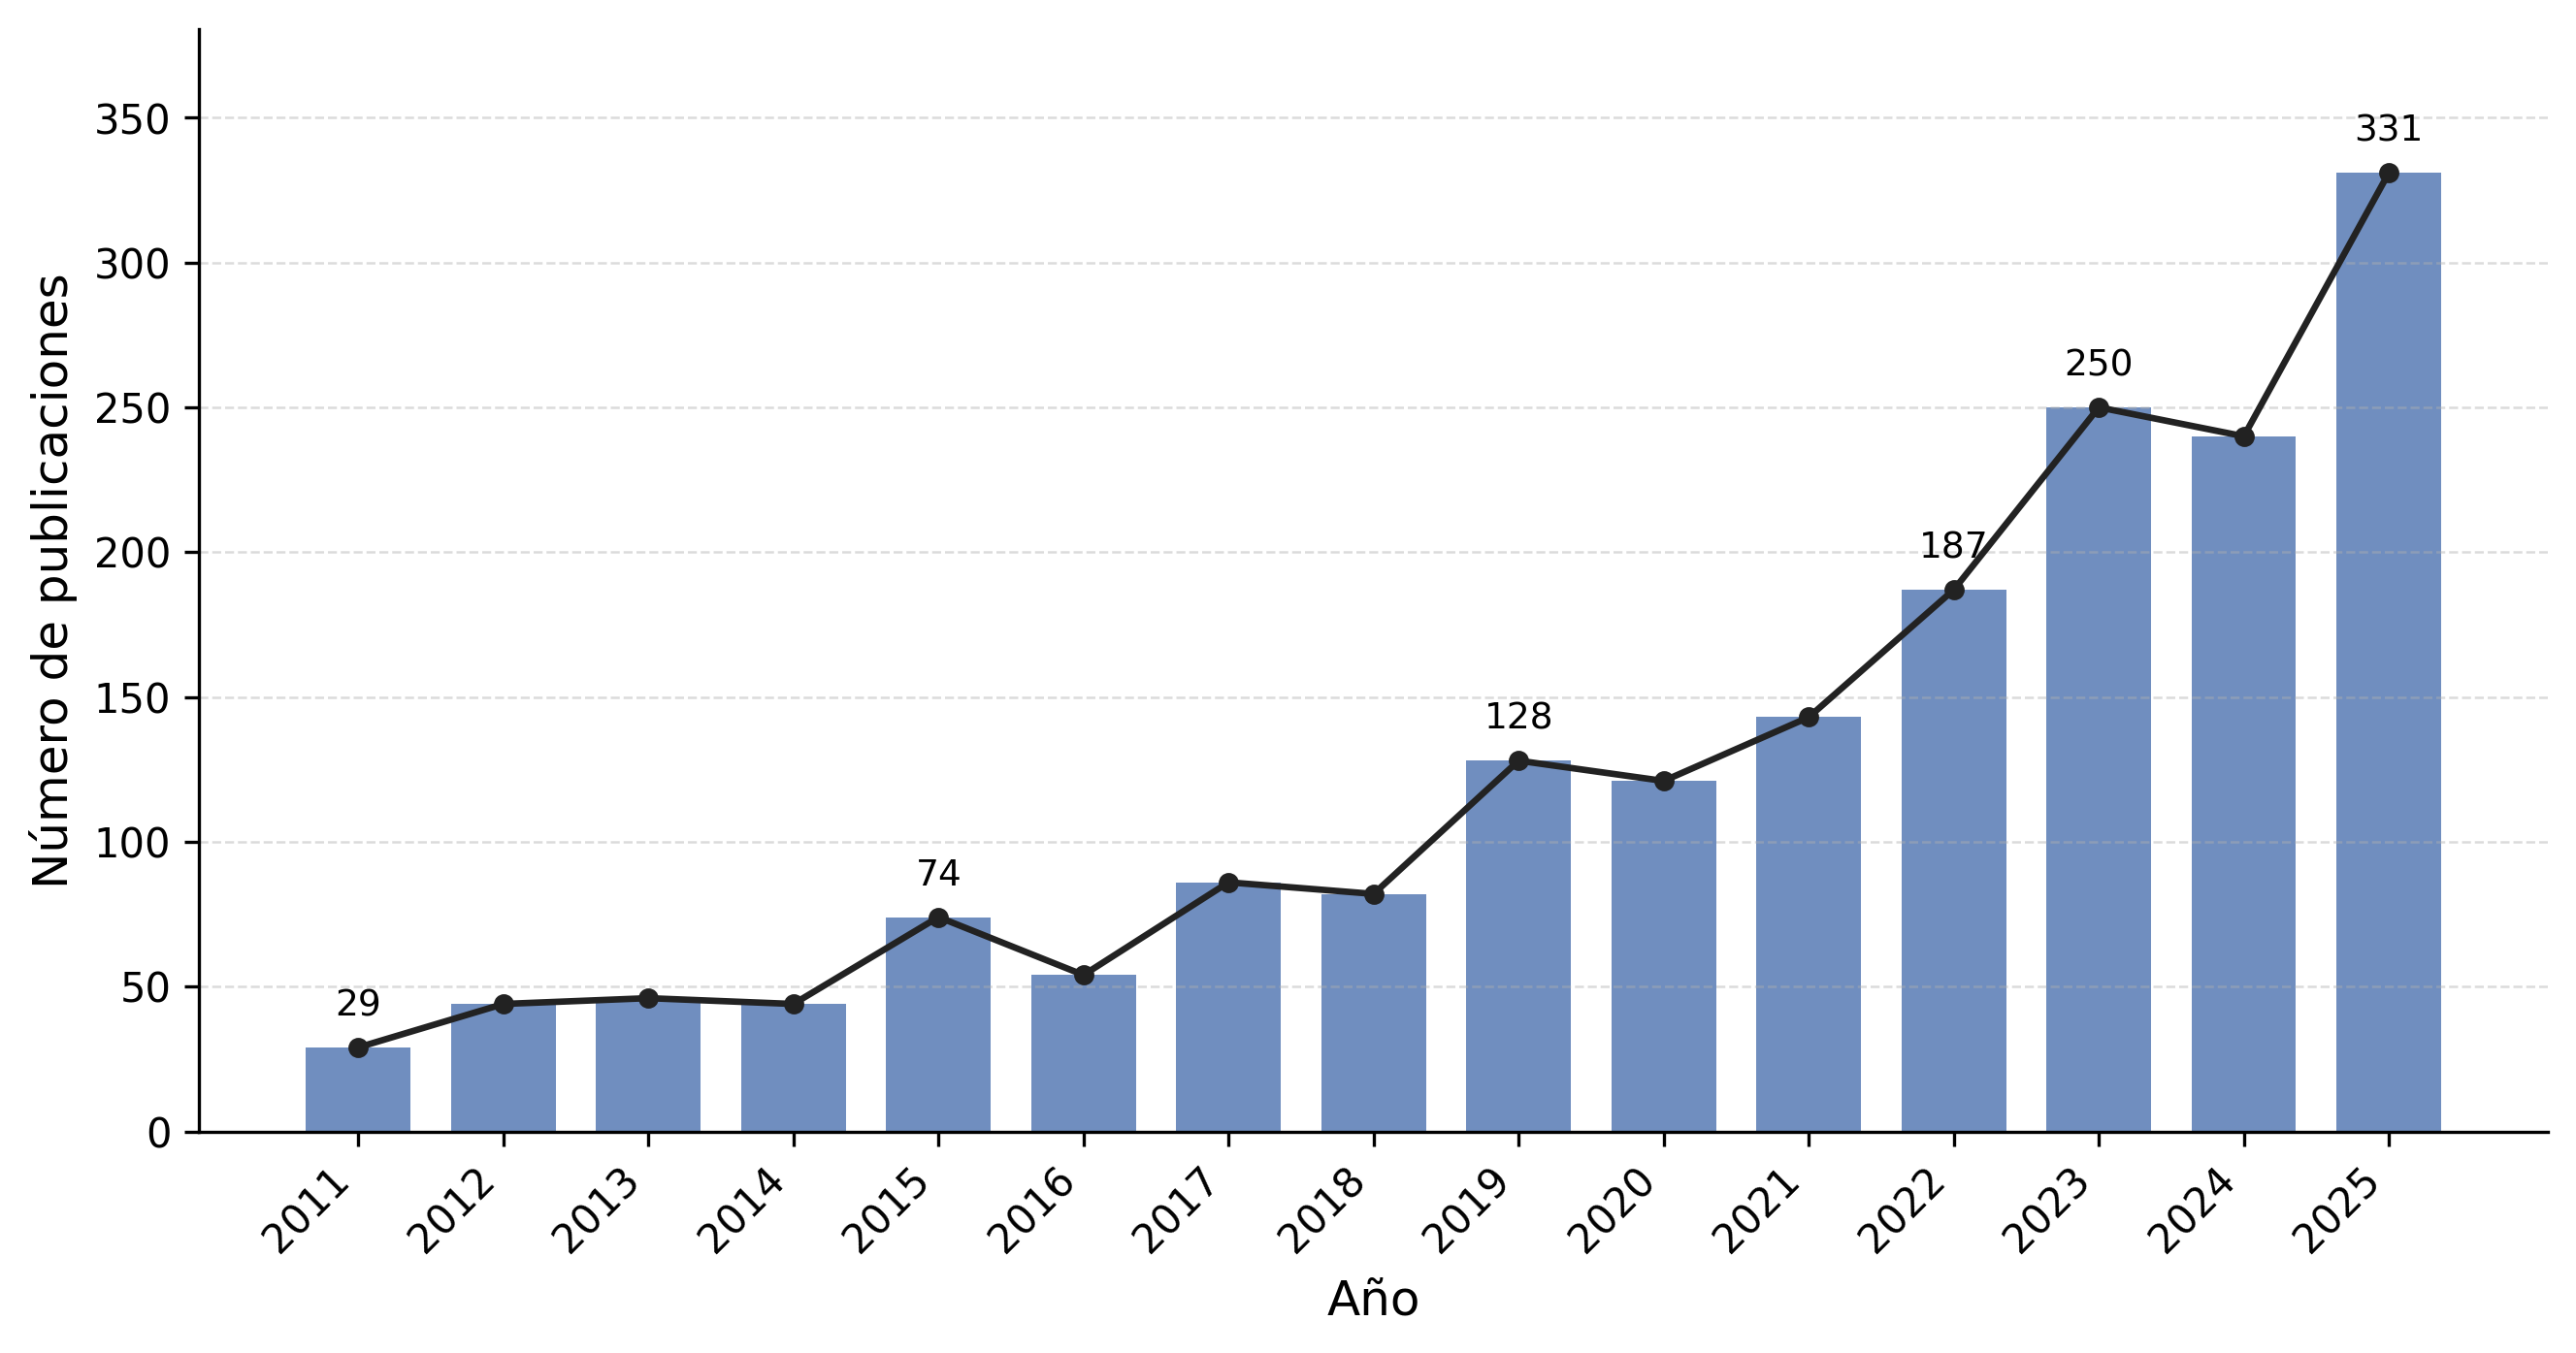
\includegraphics[width=0.85\textwidth]{figuras/estado_del_arte/publicaciones_saea_scopus.png}
    \caption{Evolución anual del número de publicaciones recuperadas en Scopus sobre algoritmos evolutivos asistidos por subrogados.}
    \label{fig:publicaciones_saea_scopus}
\end{figure}

Este capítulo sitúa la propuesta del presente trabajo dentro de esta línea de
investigación. A diferencia del capítulo anterior, centrado en los fundamentos
teóricos necesarios para comprender las técnicas empleadas, aquí el interés
recae en cómo la literatura ha abordado la integración de modelos subrogados
en algoritmos evolutivos y qué cuestiones permanecen relevantes para el diseño
experimental de este Trabajo de Fin de Grado. En particular, se presta atención
a la gestión del modelo durante la búsqueda, al tipo de información que debe
aportar el subrogado y a su integración dentro de metaheurísticas
poblacionales.  Dentro de este marco, también se considera el uso de modelos de aprendizaje automático supervisado como subrogados.

Aunque la optimización multiobjetivo asistida por subrogados constituye una
línea de investigación extensa y en auge, este trabajo se acota a la optimización
continua mono-objetivo. Esta delimitación permite centrar la revisión en los
trabajos más próximos al objetivo de esta memoria: caracterizar distintos modelos
subrogados sobre trayectorias evolutivas y estudiar posteriormente su
integración \textit{online} como mecanismo de filtrado dentro de las
metaheurísticas consideradas.

\section{Optimización evolutiva asistida por subrogados}
\label{sec:estado_saea}

El uso de modelos aproximados en optimización no es exclusivo de los
algoritmos evolutivos. Métodos como \textit{Efficient Global
    Optimization} (EGO) se apoyaron en Kriging, una técnica estadística clásica de
interpolación y modelado espacial, para guiar la búsqueda de óptimos en
funciones de caja negra costosas~\cite{jones1998}. Estas ideas sentaron una
base importante para el desarrollo posterior de la optimización basada en
subrogados dentro del cálculo computacional.

Dentro de la computación evolutiva, la incorporación de modelos subrogados se
planteó inicialmente como una forma de aproximar el \textit{fitness} de los
individuos sin evaluar siempre la función objetivo real. La revisión de
Jin~\cite{jin2005} agrupó diferentes modelos de aproximación, incluyendo
polinomios, Kriging y redes neuronales. Esta variedad refleja que los
subrogados pueden construirse tanto mediante técnicas estadísticas clásicas
como mediante modelos de aprendizaje automático supervisado. Además, este trabajo
destacó que el problema no se limita a la elección de un modelo predictivo, sino
también a decidir cómo combinar sus predicciones con evaluaciones reales para evitar que un comportamiento inadecuado del subrogado dirija la búsqueda hacia regiones incorrectas del espacio de soluciones.

A partir de estos fundamentos, años después Jin~\cite{jin2011surrogate} revisó los avances recientes de la disciplina y acotó los retos pendientes del área, entre ellos la necesidad de estrategias de gestión del modelo, el uso de varios subrogados y la falta de estudios comparativos suficientemente sistemáticos. Estos trabajos consolidan una una idea que sigue siendo crucial en la literatura actual: el subrogado no debe entenderse como un sustituto directo y permanente de la función objetivo, sino como un componente dinámico que debe ser controlado y gestionado durante el proceso evolutivo.

Las revisiones más recientes confirman la consolidación de esta línea de
investigación. He et al.~\cite{he2023review} revisan los SAEA para problemas
de optimización costosa y los organizan atendiendo tanto a los algoritmos
empleados como a sus escenarios de aplicación. Por su parte, trabajos recientes como el de Liang et al.~\cite{liang2025survey}, proponen taxonomías y esquemas generales actualiazados para describir la construcción del subrogado, su actualización y su uso dentro del algoritmo evolutivo. En conjunto, estas revisiones muestran que la integración de subrogados ha pasado de ser una técnica auxiliar a constituir una línea de investigación propia y robusta dentro de la optimización evolutiva.

\section{Gestión del modelo subrogado durante la búsqueda}
\label{sec:estado_gestion_modelo}

Uno de los aspectos más importantes en los SAEA es la forma en que se
controla la intervención del modelo subrogado durante la búsqueda. Si el
modelo se utiliza sin una política de control adecuada, sus errores pueden acumularse y
desviar al algoritmo hacia regiones que parecen prometedoras según la
aproximación, pero que no lo son al evaluarse mediante la función objetivo
real. Por este motivo, buena parte de la literatura no se centra únicamente en
mejorar la precisión del modelo, sino en diseñar mecanismos que regulen cuándo
debe intervenir y cuándo es necesario recurrir de nuevo a evaluaciones reales.

Esta idea aparece ya en el marco propuesto por Jin et al.~\cite{jin2002framework},
donde se introducen estrategias de \textit{evolution control} para combinar
evaluaciones aproximadas y reales dentro del algoritmo evolutivo. En términos
generales, estas estrategias pueden actuar a nivel de individuo, decidiendo qué
soluciones concretas se evalúan con el modelo o con la función real, o a nivel
de generación, alternando fases en las que la población se evalúa de forma
aproximada con fases de corrección mediante evaluaciones reales. Esta distinción resulta relevante porque desplaza el problema desde la elección
del modelo hacia la definición de una política de control que determine cuándo
usar la aproximación, cuándo recurrir a evaluaciones reales y a qué nivel de la
población aplicar cada decisión.

Esta gestión también afecta al tiempo durante el cual un modelo permanece
activo antes de ser actualizado. Loshchilov et
al.~\cite{loshchilov2012selfAdaptiveCMAES} propusieron una variante de CMA-ES
asistida por subrogados que ajusta \textit{online} la vida útil del modelo y
sus hiperparámetros. Aunque se trata de una metaheurística distinta a las
consideradas en esta memoria, el trabajo ilustra que la frecuencia de
actualización del subrogado forma parte del propio diseño de la integración, y
no solo de la elección del modelo predictivo.

La necesidad de controlar el modelo se ha mantenido en propuestas posteriores.
Por ejemplo, Yu et al.~\cite{yu2019restart} propusieron una estrategia de
reinicio por generaciones para un algoritmo de enjambre de partículas asistido
por un modelo RBF global. Su propuesta integra el reinicio con mecanismos de
gestión del modelo a nivel de generación y de individuo, mostrando que la
coordinación entre la dinámica de la población y el uso del subrogado puede
mejorar la búsqueda en problemas computacionalmente costosos. Este tipo de
trabajos resulta relevante para el presente Trabajo de Fin de Grado, donde se
estudia en capítulos posteriores la conveniencia de incorporar mecanismos de
reinicio en las metaheurísticas consideradas. En ese escenario, puede esperarse
que un cambio brusco en la población afecte también a la representatividad de
las muestras utilizadas para entrenar el modelo, por lo que la intervención del
subrogado debe tratarse con cautela.

Otro aspecto relacionado con la gestión del modelo es su coste computacional.
Aunque los subrogados se introducen para reducir el uso de evaluaciones reales,
su entrenamiento y predicción también consumen recursos.
Bliek~\cite{bliek2022sustainableSBO} remarca esta cuestión: no basta con
reducir el número de evaluaciones costosas, sino que debe considerarse el coste
total del proceso, incluyendo el aprendizaje del modelo y la propia
optimización sobre la aproximación. Esta observación es especialmente
importante cuando se comparan modelos de distinta complejidad, ya que una
mejora predictiva puede no compensar si introduce un coste adicional elevado.

En conjunto, estos trabajos muestran que la integración de un subrogado dentro
de una metaheurística requiere decisiones adicionales al propio modelo
predictivo. Es necesario determinar con qué datos se entrena, cuándo se
actualiza, con qué frecuencia se consulta y cómo se evita que sus errores
condicionen de forma excesiva la búsqueda.

\section{Modelos subrogados y criterios de decisión}
\label{sec:estado_modelos_informacion}

La elección del modelo subrogado no depende únicamente de su familia
estadística o de aprendizaje, sino también del tipo de información que se
espera obtener de él. En algunos enfoques, el objetivo principal es aproximar
con la mayor precisión posible el valor numérico de la función objetivo. En
otros, basta con que el modelo permita comparar soluciones, identificar
candidatos prometedores o descartar aquellos que difícilmente mejorarán la
población. Esta diferencia es especialmente relevante en algoritmos
evolutivos, donde muchas decisiones se basan en relaciones de preferencia
entre individuos más que en el valor exacto del \textit{fitness}.

%% random forest, mlps, svr...

Esta cuestión ha sido estudiada de forma explícita por Tong et
al.~\cite{tong2021surrogate}, cuyo trabajo se tomó como referencia en el
Capítulo~\ref{chap:fundamentos_teoricos} para distinguir entre modelos
orientados al \textit{fitness} absoluto y modelos orientados al
\textit{fitness} relativo. Más allá de la taxonomía, su estudio experimental
resulta relevante porque compara modelos de distinta naturaleza, como RBF,
kNN-R, RankSVM y SVC, atendiendo no solo a la calidad predictiva, sino también
al coste de construcción y predicción y a su efecto dentro de un SAEA
mono-objetivo.

De forma complementaria, Díaz-Manríquez et
al.~\cite{diaz2017metamodeling} compararon distintas técnicas subrogadas
integradas en algoritmos evolutivos, incluyendo superficies de respuesta
polinómicas, Kriging, RBF y SVR. Su análisis resulta especialmente útil en este
contexto porque no se limita a medir la precisión de las predicciones, sino que
también considera la preservación del ranking como indicador para seleccionar
modelos adecuados dentro de un proceso evolutivo. Esta conclusión refuerza la
necesidad de valorar los subrogados no solo por su error numérico, sino también
por su capacidad para mantener relaciones de orden entre soluciones candidatas.

La incorporación de técnicas de aprendizaje automático amplía este marco más
allá de los modelos estadísticos clásicos. Naharro et
al.~\cite{naharro2022regressionPairwise} comparan formulaciones basadas en
regresión, orientadas a aproximar el \textit{fitness}, con modelos pareados
que tratan directamente la comparación entre soluciones. Su estudio considera
distintos algoritmos de aprendizaje automático, incluyendo regresión
regularizada, redes neuronales, árboles de decisión, métodos de \textit{boosting}
y bosques aleatorios. Este tipo de análisis resulta útil para este trabajo
porque muestra que la utilidad de un subrogado no depende únicamente del modelo
empleado, sino también de cómo se incorporan sus predicciones dentro del
proceso de optimización.

Algunos trabajos llevan esta idea hacia modelos de clasificación, donde el
subrogado separa soluciones prometedoras y no prometedoras. Sin embargo, el presente
Trabajo de Fin de Grado se mantiene en el ámbito de modelos regresivos, ya que
cada solución candidata tiene asociado un valor real de \textit{fitness}.

Esta distinción entre aproximar valores y apoyar decisiones justifica que la
evaluación de modelos subrogados no se limite a métricas de error absoluto.
Cuando el subrogado se utiliza dentro de una metaheurística para decidir qué
candidatos merecen una evaluación real, resulta esencial medir también si
mantiene correctamente las relaciones de orden entre soluciones. Por este
motivo, en el presente Trabajo de Fin de Grado se consideran métricas de error
junto con métricas ordinales, de forma que la selección del modelo tenga en
cuenta tanto la precisión numérica como su utilidad potencial dentro del
proceso de optimización.

\section{Integración de subrogados en metaheurísticas poblacionales}
\label{sec:estado_integracion_metaheuristicas}

La integración de un subrogado dentro de una metaheurística poblacional no se
limita a entrenar un modelo externo y consultar sus predicciones. En la mayoría
de propuestas recientes, el modelo se incorpora dentro de decisiones concretas
del algoritmo, como la selección de descendientes, la identificación de regiones
prometedoras o la elección de muestras que deben evaluarse mediante la función
objetivo real. Por ello, el rendimiento final depende tanto de la calidad del
modelo como del modo en que sus predicciones modifican la dinámica de la
población.

Dentro de los SAEA recientes, la evolución diferencial aparece con frecuencia
como base algorítmica para integrar subrogados en problemas continuos. Wang et
al.~\cite{wang2019evolutionarySampling} siguen esta idea en ESAO, donde un
modelo RBF global se utiliza para preseleccionar descendientes generados por
evolución diferencial, mientras que una búsqueda local asistida por subrogado
refuerza la explotación de regiones prometedoras.

Otros trabajos han extendido esta integración mediante estructuras más
elaboradas. Cai et al.~\cite{cai2020generalizedSAEA} propusieron un algoritmo evolutivo asistido por subrogados para problemas costosos de alta dimensión, basado en un marco de algoritmo genético que combina búsqueda local mediante subrogado, actualización guiada de la población y preselección de candidatos mediante un criterio de mejora esperada. Asimismo, Wang et al.~\cite{wang2023glsade} combinaron un modelo RBF global y un modelo Kriging local dentro de una evolución diferencial asistida por subrogados, utilizando el primero para capturar tendencias globales y el segundo para explotar regiones prometedoras teniendo en cuenta la incertidumbre del modelo. Estas propuestas muestran que el subrogado no se emplea únicamente para aproximar el \textit{fitness}, sino también para regular de forma adaptativa qué zonas del espacio de búsqueda reciben nuevas evaluaciones reales.

La frecuencia y el modo de actualización del modelo durante la búsqueda también constituyen un reto crítico en los enfoques \textit{online}, dado que el reentrenamiento continuo de un aproximador conforme se acumulan datos puede convertirse en un cuello de botella computacional. Para mitigar este impacto, trabajos como el de Zhan y Xing~\cite{zhan2021fastKriging} exploran el uso de esquemas de aprendizaje incremental orientados específicamente a reducir el coste de reconstrucción del subrogado a lo largo de las iteraciones. Esta preocupación por la eficiencia temporal es un factor clave en el presente Trabajo de Fin de Grado, donde la viabilidad de la integración \textit{online} de los modelos de aprendizaje automático considerados depende directamente de mantener un coste de computación contenido.

La presencia destacada de la evolución diferencial en esta línea de investigación ha dado lugar incluso a revisiones específicas, como la de Yu et al.~\cite{yu2025sade}, centrada exclusivamente en el análisis de algoritmos de evolución diferencial asistidos por subrogados. Esta tendencia justifica que parte de la comparación experimental del presente trabajo se realice sobre DE y SHADE, dos algoritmos directamente relacionados con esta familia. No obstante, el objetivo de esta memoria no es proponer una variante específica de evolución diferencial, sino evaluar si un modelo subrogado seleccionado mediante una fase \textit{offline} puede integrarse bajo un protocolo común como filtro \textit{online} en metaheurísticas poblacionales de distinta naturaleza, incluyendo también un algoritmo genético.

\section{Posicionamiento del presente trabajo}
\label{sec:estado_posicionamiento}

La literatura revisada muestra que la utilidad de un modelo subrogado en
optimización evolutiva no depende únicamente de su precisión predictiva. Su
efecto final está condicionado por el tipo de información que aporta, por el
coste de construirlo y actualizarlo, y por la forma concreta en que sus
predicciones intervienen dentro del algoritmo evolutivo. Esta perspectiva
motiva que el presente trabajo no plantee la selección del subrogado como una
comparación aislada entre modelos, sino como una evaluación progresiva:
caracterizar primero varios modelos subrogados sobre trayectorias evolutivas ya
generadas y, a partir de esa evidencia, estudiar posteriormente su integración
\textit{online} dentro de las metaheurísticas consideradas.

Aunque existen trabajos sobre optimización evolutiva basada en datos
históricos, revisados de forma general por Jin et
al.~\cite{jin2019datadriven}, el uso \textit{offline} realizado en esta memoria
tiene un propósito distinto. En este caso, el subrogado no se emplea para
ejecutar la búsqueda, sino para caracterizar modelos sobre trayectorias ya
generadas antes de integrarlos posteriormente en el bucle de optimización.

A partir de esa caracterización, la integración \textit{online} se aborda como
un mecanismo de filtrado controlado. El subrogado no sustituye de forma
definitiva a la función objetivo, sino que decide qué candidatos parecen lo
suficientemente prometedores como para consumir una evaluación real. De este
modo, el trabajo se sitúa en la línea de los SAEA que combinan predicción,
gestión del modelo y evaluación real, analizando hasta qué punto una misma
estrategia de integración puede aplicarse de forma robusta a distintas
metaheurísticas poblacionales consideradas en la memoria.

Los capítulos siguientes presentan las metaheurísticas, los modelos, las estrategias de evaluación y el marco experimental utilizados.

